
% Lecture Template for FE Exam Review Tristan Hill - Spring 2020 - Fall 2020 - Spring 2021
% FE Exam Revfiew 
% Chapter 8 - Dynamics  
% Lecture 1 - Overview

% Document settings

%\documentclass{beamer}                  % for presentation ?
\documentclass[handout]{beamer}  % for handout ?
\usepackage{beamerthemesplit}
\usepackage{amsmath}
\usepackage{listings}
\usepackage{multicol}
\usepackage{framed}
\usepackage{amsmath, nccmath}
\usepackage{geometry}
\usepackage{bm}

\beamertemplateballitem

\definecolor{TTUpurple}{rgb}{0.3098, 0.1607, 0.5176} % TTU Purple (primary)
\definecolor{TTUgold}{rgb}{1.0000, 0.8666, 0.0000} % TTU Gold (primary)

\setbeamercolor{palette primary}{bg=TTUpurple,fg=TTUgold}
\setbeamercolor{palette secondary}{bg=black,fg=TTUgold}
\setbeamercolor{palette tertiary}{bg=black,fg=TTUpurple}
\setbeamercolor{palette quaternary}{bg=TTUgold,fg=black}
\setbeamercolor{structure}{fg=TTUpurple} % itemize, enumerate, etc
\setbeamercolor{section in toc}{fg=TTUpurple} % TOC sections

% custom colors
\definecolor{TTUpurple}{rgb}{0.3098, 0.1607, 0.5176} % TTU Purple (primary)
\definecolor{TTUgold}{rgb}{1.0000, 0.8666, 0.0000} % TTU Gold (primary) 
\definecolor{mygray}{rgb}{.6, .6, .6}
\definecolor{mypurple}{rgb}{0.6,0.1961,0.8}
\definecolor{mybrown}{rgb}{0.5451,0.2706,0.0745}
\definecolor{mygreen}{rgb}{0, .39, 0}
\definecolor{mypink}{rgb}{0.9960, 0, 0.9960}

% color commands
\newcommand{\R}{\color{red}}
\newcommand{\B}{\color{blue}}
\newcommand{\BR}{\color{mybrown}}
\newcommand{\K}{\color{black}}
\newcommand{\G}{\color{mygreen}}
\newcommand{\PR}{\color{mypurple}}
\newcommand{\PN}{\color{mypink}}
\newcommand{\OR}{\color{orange}}
\newcommand{\GD}{\color{TTUgold}}


\newcommand{\Lagr}{\mathcal{L}} % lagrangian

\newcommand{\hspcu}{\underline{\hspace{20mm}}} % large horizontal space w underline
\newcommand{\vspccc}{\vspace{6mm}\\} % large vertical space
\newcommand{\vspcc}{\vspace{4mm}\\}   % medium vertical space
\newcommand{\vspc}{\vspace{2mm}\\}     % small vertical space

\newcommand{\hspcccc}{\hspace{10mm}} % large horizontal space
\newcommand{\hspccc}{\hspace{6mm}} % large horizontal space
\newcommand{\hspcc}{\hspace{4mm}}   % medium horizontal space
\newcommand{\hspc}{\hspace{2mm}}     % small horizontal space

\newsavebox{\mybox} % custom box

%\newcommand{\MNUM}{1\hspace{2mm}} % Module number
%\newcommand{\CNUM}{7\hspace{2mm}} % Chapter number 
\newcommand{\moduletitle}{FE Exam Review} % Titles and Stuff
\newcommand{\topictitle}{Chapter 8 Dynamics - Lecture 1} 

\newcommand{\sectiontitleI}{Introduction to Dynamics} % More Titles and Stuff
\newcommand{\sectiontitleII}{Kinematics of a Particle}
\newcommand{\sectiontitleIII}{Rigid Body Kinematics}
\newcommand{\sectiontitleIV}{Newtons Laws of Motion}
\newcommand{\sectiontitleV}{Examples}


\author{Tristan Hill (thill@tntech.edu)}
\title{\moduletitle}
\date{Mechanical Engineering\vspc Tennessee Technological University}

\begin{document}

\lstset{language=MATLAB,basicstyle=\ttfamily\small,showstringspaces=false}

\frame{\titlepage \center\begin{framed}\Large \textbf{\topictitle}\end{framed} \vspace{5mm}}

% Section 0 - Outline
\frame{
	
	\large \textbf{\topictitle} \vspace{3mm}\\
	\begin{multicols}{2}
	\begin{itemize}
	
		\item \sectiontitleI    \vspc % Section I
		\item \sectiontitleII 	\vspc % Section II
		\item \sectiontitleIII 	\vspc %Section III
		\item \sectiontitleIV 	\vspc %Section IV
		\item \sectiontitleV 	\vspc %Section V
	
	\end{itemize}
    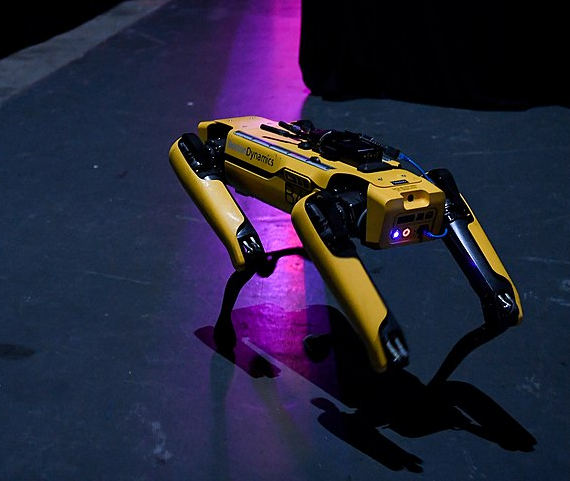
\includegraphics[scale=.225]{spotmini_cropped.png}
	{\tiny image: \href{https://www.flickr.com/photos/websummit/49028927416/}{wikimedia-commons(flickr)} }
	\end{multicols}	
	
	{\small Also in Ch. 8

	\begin{itemize}
		\item Work and Energy Methods
		\item Kinetics of Rigid Bodies
	\end{itemize}
}
}


\section{\sectiontitleI}

\frame{
  \frametitle{\sectiontitleI}
  			
  \textbf{What is Dynamics?}\\		
			
    \begin{itemize}
    	
    	\item {\bf Dynamics} is a subset of mechanics focused on the motion of bodies and the forces that affect them. \vspace{5mm}
		
		\item .. fundamental to many disciplines of engineering. \vspace{5mm}
		
		\item .. essential in {\bf mechanical engineering} and {\bf design}.

	\end{itemize}  

}

\section{\sectiontitleII}

\frame{
	\frametitle{\sectiontitleII}
  
We begin with a particle (point mass) moving in space. \\

\[\vec{v}=\frac{d\vec{r}}{dt}=v\hat{e_t}\]

\[\vec{a}=\frac{d\vec{v}}{dt}=\dot{v}\hat{e_t}+\vec{v}\frac{ds}{dt}\frac{d\hat{e_t}}{ds}=\dot{v}\hat{e_t}+\frac{\nu^2}{\rho}\hat{e_n}\]

\[\frac{d\hat{e_t}}{ds}=\kappa \hat{e_n} \]

}

\frame{
	\frametitle{\sectiontitleII}
	
Distance Velocity and the Tangential Component of Acceleration \\

\[\frac{d{v}}{dt}=a_t \hspace{10mm} or \hspace{10mm} v=v_0+\displaystyle\int a_tdt\]
\[\frac{d{s}}{dt}=v \hspace{10mm} or \hspace{10mm} s=s_0+\displaystyle\int vdt\]

\[v\frac{dv}{ds}=a_t \] 
\[v^2=v_0^2+2\displaystyle\int a_tds\]

}

\frame{
	\frametitle{\sectiontitleII}
	
Constant Tangential Acceleration \\

\[v=v_0+a_tt\]

\[s=s_0+v_0t+\frac{1}{2}a_tt^2\] 

\[v^2=v_0^2+2a_ts\]

}

\section{\sectiontitleIII}

\frame{
  \frametitle{\sectiontitleIII}
	
	
Rigid Body Kinematics \vspace{5mm}

Constraint of Rigidity \vspace{5mm}

\[ \frac{d}{dt}|r_{pq}|^2=\frac{d}{dt}(\vec{r}_{pq}\cdotp\vec{r}_{pq})=2\vec{r}_{pq}\cdotp\frac{d\vec{r}_{pq}}{dt}=0 \] \vspace{5mm}

Instantaneous Zero Velocity \\

	

}
\section{\sectiontitleIV}

\frame{
  \frametitle{\sectiontitleIV}
  
   Newtons Laws of Motion \vspcc
   {\it Every object persists in its state of rest or uniform motion in a straight line unless it is compelled to change that state by forces impressed on it.} \vspcc
   
   {\it Force is equal to the change in momentum ($mV$) per change in time. For a constant mass, force equals mass time acceleration ($F=ma$).}\vspcc
   
   {\it For every action, there is an equal and opposite re-action.}\vspcc
   
   
}

\frame{
	\frametitle{\sectiontitleIV}
   \[\vec{f}=m\vec{a}\]
   
   \[\vec{p}=\displaystyle\Sigma_i m_iv_i\]
   
   \[\frac{d\vec{p}}{dt}=\displaystyle\Sigma_i m_ia_i\]
   

}


\section{\sectiontitleV}

\frame{
  \frametitle{\sectiontitleV}	

 	Example 1 (Ex. 8.8): \\
 	\begin{multicols}{2}
 	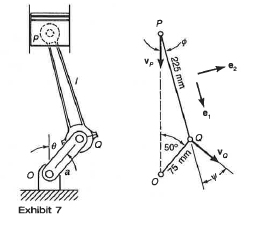
\includegraphics[scale=0.8]{piston_cropped.png}
 	\small
 	As the crank OQ in Exhibit 7 rotates clockwise at 200 rad/s, the piston P moves vertically. What will be the velocity of the piston at the instant when the angle $\theta$ is 50 degrees?
 	\end{multicols}
 	 \vspace{20mm}
  
}

\frame{
	\frametitle{\sectiontitleV}	
	
	Example 1 (cont.): \\
		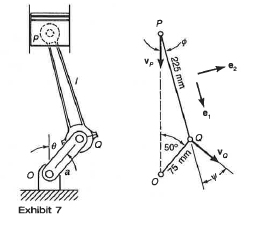
\includegraphics[scale=0.8]{piston_cropped.png}


	\vspace{20mm}
	
}

\frame{
	\frametitle{\sectiontitleV}	
	
	Example 2 (Problem 8.9): \\
	\begin{multicols}{2}
		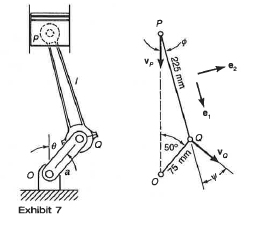
\includegraphics[scale=0.8]{piston_cropped.png}
		\small
	What will be the angular velocity of the connecting rod in Example 8.8, at the instant when the angle $\theta$ is 50 degrees?
	\end{multicols}
	\vspace{20mm}
	
}

\frame{
	\frametitle{\sectiontitleV}	
	
	Example 2 (cont.): \\
	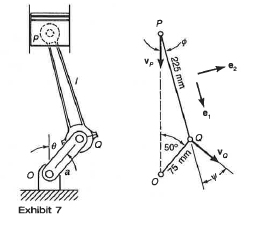
\includegraphics[scale=0.8]{piston_cropped.png}
	
	
	\vspace{20mm}
	
}

 
\frame{
	\frametitle{\sectiontitleV}	
	
	Additional Examples (cont.): \\
		\begin{multicols}{2}
		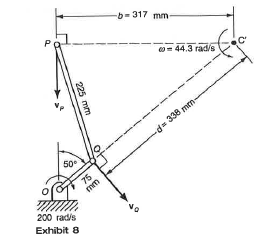
\includegraphics[scale=0.8]{example_8_10b_croppedA.png}
		\small
		What is the location of the instantaneous center C' of the connecting rod in Examples 8 and 9? use this to verify the previously-determined values of the angular velocity of the connecting rod and the velocity of point P.
	\end{multicols}
		
	\small
	
	\vspace{20mm}
}

\frame{
	\frametitle{\sectiontitleV}	
	
	Example 3: \\
	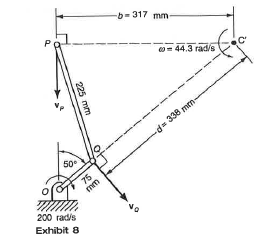
\includegraphics[scale=.8]{example_8_10b_croppedA.png}
	
	\small
	
	
	\vspace{20mm}
	
}
\frame{
	\frametitle{\sectiontitleV}	
	
	\small{Solutions to Example 1 (Ex. 8.8):} \\
	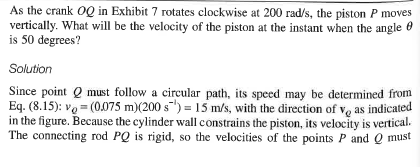
\includegraphics[scale=1.0]{example_8_8.png}
	\small
	
	\vspace{20mm}
	
}

\frame{
	\frametitle{\sectiontitleV}	
	
	\small{Solutions to Example 1 (Ex. 8.8) (cont.):} \\
	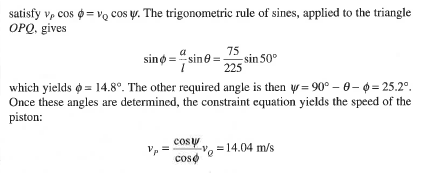
\includegraphics[scale=1.0]{example_8_8b_cropped.png}
	\small
	
	\vspace{20mm}
	
}

\frame{
	\frametitle{\sectiontitleV}	
	
	\small{Solutions to Example 2 (Ex. 8.9):} \\
	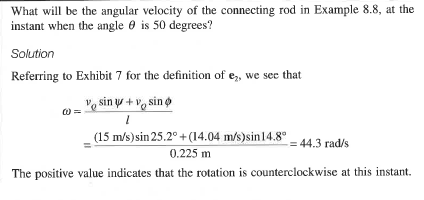
\includegraphics[scale=1.0]{example_8_9.png}
	\small
	
	\vspace{20mm}
	
}

\frame{
	\frametitle{\sectiontitleV}	
	
	\small{Solutions to Example 3 (Ex. 8.10):} \\
	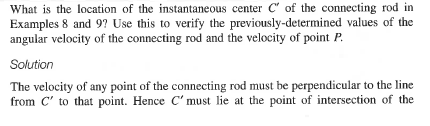
\includegraphics[scale=1.0]{example_8_10.png}
	\small
	
	\vspace{20mm}
	
}

\frame{
	\frametitle{\sectiontitleV}	
	
	\small{Solutions to Example 3 (Ex. 8.10) (cont.):} \\
	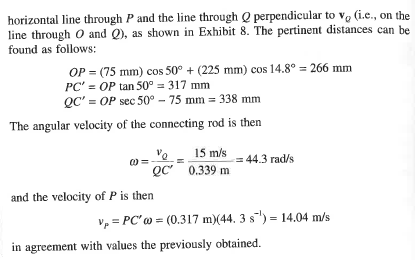
\includegraphics[scale=1.0]{example_8_10b_cropped.png}
	\small
	
	\vspace{20mm}
	
}

\frame{
	\frametitle{\sectiontitleV}	
	
	\small{Solutions to Example (Ex. 8.10) (cont.):} \\
	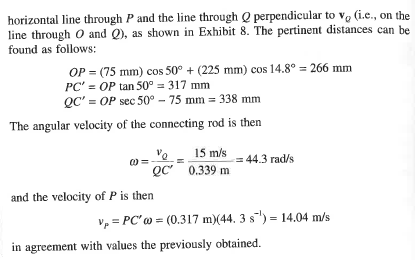
\includegraphics[scale=1.0]{example_8_10b_cropped.png}
	\small
	
	\vspace{20mm}
	
}  
  
  
\end{document}
